\chapter{Implementation}


\section{Hierarchy of Arrays}

The API of an array is defined by an interface called \textit{INDArray} which has a dense implementation for each backend: \textit{NDArray} class for the CPU and \textit{JCublasNDArray} class for the GPU. But since most of the operations and methods are shared between the two backends, they are implemented in an abstract class called \textit{BaseNDArray}.

Adding sparse representations asked two questions:
\begin{enumerate}
 	\item What can be shared with the dense arrays ?
	\item What can be between the different sparse arrays and what are format-specific ?
\end{enumerate}

To answer those questions, we need to go a little bit deeper in the implementation. 

The dense implementation includes methods that are inherently related to the way dense array is internally made, and other methods are related to the generic parameters such as the shape or are utility method.

The first type of methods is not useful in case of sparse. Dense and sparse arrays are not built in the same manner. Methods such as \textit{getStrides} are not relevant in the sparse context. Reciprocally the sparse array will need methods which will be irrelevant in the dense context.

We encounter the same situation between the different sparse formats. Some will need utility methods that the other ones won't need.

But everything has to be defined in the \textit{INDArray} interface. To avoid code duplication, everything than can be shared should be implemented in the higher level of the hierarchy. The methods that are not compatible with a type of array will simply throw an unsupported operation exception.

The drawback brought with this solution is that we always need to verify the type of the array before doing any operations.

// TODO update schema
 
\begin{figure}[H]
	\begin{center}
	%	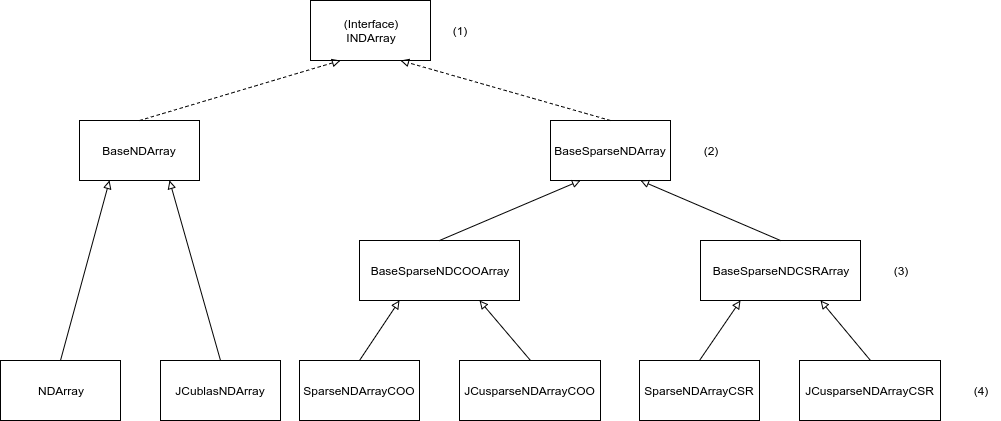
\includegraphics[width=6.5in]{images/INDArrayHierarchy.png} 
		\label{fig:hierarchy}
		\caption{Arrays hierarchy in Nd4j}
	\end{center}
\end{figure}


\section{Limitations and Constraints}

Nd4j has been made in the perspective of dense arrays. The design has been thought and optimized regarding the dense implementation which brings some constraints to implement the sparse representation
\subsection{storing off-heap}

// TO ASK TO RAVER

What are the advantages for storing data off-heap ? Why Garbage collector is a bad thing ?

What the idea behind workspaces and how does it work ?

Before the workspaces, data were already stored off-heap. What do workspaces bring new ? 

Why it wasn't possible to have arrays of databuffers native side ? what we had to flatten everything?

Why didn't we use managed memory?

\subsection{Workspaces}
\subsection{DataBuffers have a fixed length}

Databuffers cannot be reallocated -> necessary in case of sparse
-> explain the reallocation mechanism

--------
-> we can reallocate memory from java side but it's impossible from native side. so we need to overallocated to the max result size before any operations !

1 - estimate the size needed (only the size of the view -> which avoid to allocated at the max size of the array - it wouldn't fit in memory)
2 - reallocate
3 - perform the op

-> add in op interface

We also overallocate by a factor 2 the size of the databuffers used for storing the values and the indexes -> avoid too much reallocation

\subsection{Alternatives}
-> TODO %TODO            better explaination
The implementation of CSR and COO would have been easier with managed memory. We could have stored the arrays in Java ArrayList and we woudn't have to take care of the memory, reallocation, etc 


\section{CSR Matrices}
\subsection{Structure}

The representation uses 4 data buffers to encore a CSR matrix. One for the non-zero values, one for the columns indexes and two for the row pointers (to the beginning and to the end of each row).

\subsection{Put a value}

To insert a new value or to update an existing non-null value, we need to identify where the values of row we want ot insert to are located in the values buffer and in the columns buffer. The beginning and end of rows pointers give us the range of indexes.

While iterating over the range of values, if we find a value with the same column index than the one we want to insert to, we can update the values and nothing needs to be changed in the three other buffer. 

However if there is no value with that column, we need to insert a new one at the correct position. Then we need to update the end of row pointer for this row. Finally each row pointers that come after need to be increment by one.

% TODO
-- ADD pseudo code for putscalar of csr?



\subsection{Get a Sub-array}

\begin{enumerate}
\item First, we need to resolve the index to get the new shape of the array, the new rank, etc. In the case we use the resolution of the dense array but we are only interested in
\begin{itemize}
	\item the shape: an array with two elements containing the new shape of the sub-array.
	\item the offsets: an arays with two elements that indicate the first row and the first column that belongs to the sub-array.
	\item the offset: indicates the position in the data buffer of the first element that belongs to the sub-array.
\end{itemize}
 \item Sometimes the offsets are equals to zeros while having a non-null offset. In this case we need to override the offsets.
\begin{lstlisting}
	 offsets[0] = (int) resolution.getOffset() / shape()[1];
	 offsets[1] = (int) resolution.getOffset() % shape()[1];
\end{lstlisting}
\item With the offsets we can now compute the first and the last position of each dimension.
\begin{lstlisting}
	long firstRow = offsets[0];
	long lastRow = firstRow + shape[0];
	long firstColumn = offsets[1];
	long lastColumn = firstElement + shape[1];
\end{lstlisting}
\item Now we have the bounds for each dimension, we can reconstruct the new beginning and end of row pointers et the columns indexes.
\end{enumerate}

% put the code in annex?

\subsection{Limits of this format}

This formats only works with two dimensions and cannot be extended to tensors. Therefor it makes it difficult to be compatible with the API.
Moreover the operations to get or put values aren't straightforward. Several step are necessary before accessing the value.

\section{COO Tensors}
\subsection{Naive implementation} \label{ssec:naiveCoo}

Based on the description in \ref{sssec:coo} the COO encoding needs one data buffer to store all the non-null values and one for the indexes of each values. 

An easy solution would have been to store the indexes into a multi-dimension array of \textit{DataBuffers}: One buffer for each value, or one buffer for each dimension. Due to the native constraints that makes hardly manageable to have such arrays (Difficulty to pass the array to the native side and Cuda side), we choose to flatten the indexes into one buffer.

\begin{figure}[!h]
	\subfloat[each index is stored contiguously]{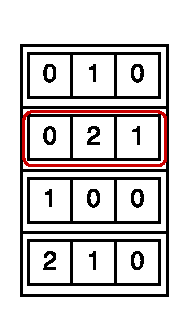
\includegraphics[width=1.5in]{images/indexesCoo_a.pdf} \label{fig:cooIdxA}}
	\subfloat[Each dimension is stored contiguously]{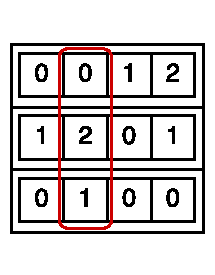
\includegraphics[width=1.5in]{images/indexesCoo_b.pdf} \label{fig:cooIdxB}}
	\subfloat[Flattened Indexes]{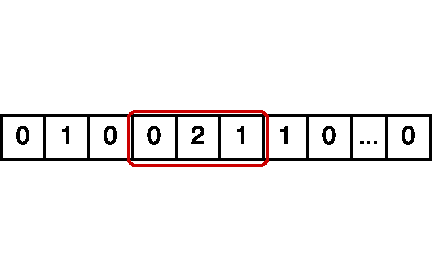
\includegraphics[width=2.5in]{images/indexesCoo_c.pdf} \label{fig:cooIdxC}}
	\hfill
	\caption{Illustration of the different possible datastructure for storing the indexes  [0, 2, 1] of a value $v$ }
\end{figure}

% TODO regenerate the schema - too much bottom margin

But this implementation makes difficult to be compliant with the API. It brings several issues:
\begin{itemize}
	\item The key of views is the sharing of their data. In case of COO format, views have to share the data buffer and the indexes buffer. Without the indexes it is not possible to add a value in the original array by adding it in a view. If we only put the new value in the shared value buffer without updating the indexes, the original array would have a value buffer bigger than its indexes buffer and there would be an offset between the values and the indexes. 
	
	Even when sharing both buffers, how would we know which value is included in the view and which is ot? 	
	
	\item The coordinates of a value in a view are not necessary the sames of the same value in the original array. 
		
	They can be offset if dimension is partially included in the view. Figure \ref{fig:viewOffset} shows a matrix an a view (in red). The value$ v_{i}=5$ would have the coordinates [1, 1] in the original array while it has the coordinates [0, 0] in the view. How the indexes can be translated between views?
	\begin{figure}[!h]
		\centering
		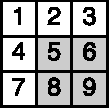
\includegraphics[width=0.8in]{images/viewIndexOffset.pdf}
		\caption{A $3\times 3$ matrix with a $2\times 2$ view in grey}
		\label{fig:viewOffset}
	\end{figure}

	\item A view can have a lower or higher rank than its original array. How can the view indexes be stored ?
\end{itemize}

\subsection{More parameters are needed to define the tensors}

Most of the issues cited in section \ref{ssec:naiveCoo} are due to the support of the different types of indexes. Each index implements the interface \textit{INDArrayIndex} and extends from \textit{NDArrayIndex}. They provide a very efficient and powerful mechanism to access part of a array but they introduce some constraints when implementing views for COO.

\subsubsection{All Indexes}
\textit{All} indexes are the most straightforward of the library. They are used to collect all the elements of a dimension.

\subsubsection{Interval Indexes}
\textit{Interval} indexes takes an subpart of a dimension containing in an interval. They don't modify the rank

The grey sub-array in figure \ref{fig:viewOffset} is the result of the operation :
\begin{lstlisting}
	myArray.get(NDArrayIndex.interval(1, 3), NDArrayIndex.interval(1, 3));
\end{lstlisting} 
After the resolution of the indexes, we obtain offsets equal to $[1, 1]$ with an offset equals to $4$.
In the COO perspective that means a value having any of its dimensions equal to 0 does not belong to the view. We need to define bounds for each dimension in order to be able to filter out the values.

\subsubsection{Point Index}
\textit{Point} indexes take one unique element of a dimension. They reduce the rank of the array.

\begin{figure}[!h]
	\centering
	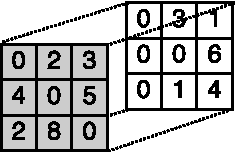
\includegraphics[width=1.5in]{images/tensorsHiglighted.pdf}
	\caption{Result of \textit{get(point(0), all(), all())} on the first dimension in grey on a $2\times 3\times 3$ tensor}
	\label{fig:pointTensor}
\end{figure}

Figure \ref{fig:pointTensor} shows a $2\times 3\times 3$ tensors with a $2\times 2$ matrix view which is the result of the operations:
\begin{lstlisting}
	myArray.get(NDArrayIndex.point(0));
\end{lstlisting} 

The coordinates of the resulting matrix have only two dimensions instead of three. We have an issue when trying to access a value given a pair of coordinates in the view context. There is no direct matching between these coordinates and those who actually are in the indexes buffer. 

The solution is to add an additional parameter array that keeps track of the status of each dimension. 
The array is called flags and it can contains either 0, which means \textit{active}, or 1 which means \textit{fixed}. The flags array for the view shown in figure \ref{fig:pointTensor} would be equal to [1, 0, 0] because the first dimension is fixed at position 0.

\subsubsection{Specified Index}
When using at least one specified index in the set of indexes used to get a sub-array, it always returns a copy of the original data. It can not be a view because the specified indexes are not deterministic and can not be translated into logical strides, shape or offsets.

In this case we need to iterate over each dimension to access every element of the array and test if the current value belongs to the view. If it is the case, we add it in a new array. We are still using the indexes resolution to get the new shapes, the offsets, etc.


\subsubsection{New Axis Index}
\textit{New axis} indexes are used to add a new dimension to the array. The new dimension always has a length equals to 1. It can be perpended or inserted in the middle of the dimensions.
Since the rank is higher, more coordinates are needed to access a value. However the shared indexes buffers is limited to the original rank. Similarly to the point index, we need a new parameter array that keep tracks of the position of the new dimensions to be able to  translate the coordinates from view to original context.

Assuming we have a $3\times 3$ matrix: calling \textit{myArray.get(NDArrayIndex.newAxis())} will prepend a new dimension. The view is a $1\times 3\times 3$ tensor with a hidden dimension parameter array equal to $[0]$.


\subsection{Computations of the the Parameters}
\subsubsection{Computation of the Sparse Offsets}

The sparse offsets are computed from the offset. The offset give us the position of the first element in the array. We want to reverse it the coordinates of this values which will be the sparse offset. 


\begin{enumerate}
	\item For each dimension except the innermost one, we divide the offset by the number of elements in one dimension's element (i.e divide the offset by the number of value in a row). Rounded to the lower integer, this quotient give us the sparse offset for the dimension. Then we need to remove the number of elements that are in the same dimension but at a lowest value. We want to isolate the dimension's value as if it was the value 0 of the dimension.
	\item We iterate until the last element. In this case we have the offsets set up up to the row dimension. To find which column the value is in, we need to take the modulo of the remaining offset by the number of columns.
	\item We have the sparse offsets given a set of indexes. But it does not take into account the possibly already non-null sparse offsets. This is the case when we take a view from a view. In this case we need to merge the two sparse offsets arrays. The final result is the sum of the existing offset and the freshly computed offset.
	\item We should particularly be careful with fixed dimensions because they are absent from the sparse offset resolution explained above. The result does not contain any information about them, we need to merge them in a new array which has a length equals to the underlying rank. In this case, it takes the value of the existing offset.

\end{enumerate}

\begin{algorithm}
	\caption{Calculate the sparse offsets}
	\label{alg:sparseOffsets}
\begin{algorithmic}
	\Statex
	\Procedure{CreateSparseOffsets}{int $offset$}\\
	\Comment{$rank$, $underlyingRank$, $shape$ and $sparseOffsets$ are class fields}\\
	\State $newOffsets\gets new\ int[rank]$ \Comment{Compute the new offsets}
	
	\For{$i=0$ to $(rank - 2)$} 
	\State $nbElements \gets \prod_{j=i+1}^{rank} shape[j]$
	\State $newOffsets[i] \gets \lfloor offset \div nbElements\rfloor$
	\State $offset \gets offset - newOffsets[i] \times nbElements$
	\EndFor
	\State $newOffsets[rank-1] \gets offset \mod shape[rank-1]$ 
	\\
	\\	
	\State $finalOffsets\gets new\ int[underlyingRank]$	\Comment{Merge with sparseOffsets of this array}
	\State $active\gets 0$
	\For{$i=0$ to $underlyingRanke$}
	\If {$flags[i] == 0$}
	\State $finalOffsets[i] \gets sparseOffsets[i]$
	\Else
	\State $finalOffsets[i] \gets newOffsets[active] + sparseOffsets[i]$
	\State $i \gets i + 1$
	\EndIf
	\EndFor\\
	\Return $finalOffsets$
\EndProcedure
\end{algorithmic}
\end{algorithm}
	

\subsubsection{Computation of the Flags}
Flags determine which dimension is active and which one is hidden from the point of view of the array. The dimension can only be reduced with point index, which means the flags can be computed during the offset resolution. We fill the flags array while iterating over the indexes array.

\subsubsection{Computation of the Hidden Dimensions}

The resolution returns an array containing the position of the \textit{newAxis} indexes in the indexes array. The array may already have some hidden dimensions. In this case we need to adapt the result with the current hidden dimension.

\begin{algorithm}
	\caption{Calculate the hidden dimensions}
	\label{alg:hiddenDim}
	\begin{algorithmic}
			
		\Procedure{CreateHiddenDimensions}{int[] $newAxis$}\\
		\Comment{$hiddenDimensions$ is a class field}\\
		
		\If {$newAxis$ is empty or null}
		\Return {$hiddenDimensions$}		
		\EndIf
		\\
		\If {$hiddenDimensions$ is empty}
		\Return {$newAxis$}		
		\EndIf
		\\	
		
	
		\State $size\gets newAxis.length + hiddenDimensions.length$ 	\Comment{Merge both arrays}
		\State $newArray \gets $ new $int[size],\ i\gets 0,\ newDim\gets 0$
		\\
		\For{$oldDim=0$ to $hiddenDimensions.length$}
			\State $j\gets 0$
			\While{$newAxis[newDim] < hiddenDimensions[i]$}
				\State $newArray[i] \gets newAxis[newDim]$
				\State $i\gets i + 1,\ j\gets j + 1$ 	
			\EndWhile
			\State $newArray[i] \gets hiddenDimensions[oldDim] + j$	
			\Comment{add an offset corresponding to the amount of axis added before this dimension}
			\State $i\gets i + 1$
		\EndFor
		\Return{$newArray$}
		\EndProcedure
	\end{algorithmic}
\end{algorithm}


\subsection{Sparse Indexes Translation}

To translate a view coordinates to the underlying coordinates, we have to take into accounts: the sparse offsets, the hidden dimensions and the flags. With those three parameters we have everything need for translating.
	
While iterating over the view dimensions, three situations can happen :
\begin{enumerate}
	\item The current dimension is hidden: We do nothing
	\item The current dimension is fixed: We put the corresponding offset into the result array. Since several fixed dimensions can occur in a row, we need to repeat until we reach an active dimension.
	\item The current dimension is active: We sum the view coordinate with the sparse offset.
\end{enumerate}
This method is described in detail in algorithm \ref{alg:translation} 
	
	
\begin{algorithm}
	\caption{Translate the indexes from view to underlying context}
	\label{alg:translation}
	\begin{algorithmic}
		
		\Procedure{translate}{int[] $viewIndexes$}\\
		\Comment{$underlyingRank$, $hiddenDimensions$ and $sparseOffsets$ are class fields}\\
		\State $result \gets new\ int[underlyingRank]$
		\State $idxPhy \gets 0,\ hidden \gets 0 $
		\\
		\For{$idxVir=0$ to $viewIndexes.length$}\\
		
		 \Comment{The current dimension is hidden, it does not appear in the result}
			\If{$hidden < hiddenDimension.length \And hiddenDimension[hidden] == idxVir$}
				\State $hidden \gets hidden + 1$
			\Else
				\While{$idxPhy < underlyingRank \And isFixed(idxPhy)$}
					\State $result[idxPhy] \gets sparseOffsets[idxPhy]$ \Comment{If the dimension is fixed, the coordinate takes the value of the offset}
					\State $idxPhy \gets idxPhy + 1$
				\EndWhile\\
				\Comment{If the dimension is not fixed, we add the offset to the coordinate}				
				
				\If{$idxPhy < underlyingRank \And  !isFixed(idxPhy)$}
					\State $result[idxPhy] \gets sparseOffsets[idxPhy] + viewIndexes[idxVir]$ 
					\State $idxPhy \gets idxPhy + 1$
				\EndIf
		
			\EndIf
			
		\EndFor		
		\EndProcedure
		\end{algorithmic}
	\end{algorithm}
	
\subsection{Included values}



\subsection{?}
binary search to reverse the indexes 

tensor contractions not equals depending on the dimensions because the time to access the elements is not the same because the values are sorted along the first dimension
-> binary search, skip list, tree ...

\subsection{Final Implementation}
	
	The final representation is encoded with 5 \textit{DataBuffers}:
	\begin{enumerate}
		\item Values: Stored the value linearly.
		\item Indexes: Stored the flattened indexes of each values.
		\item Flags: Define which dimensions are active and which are fixed.
		\item Sparse Offsets: Define the bound of each dimension.
		\item Hidden Dimensions: Keep track of the position in the shape array of the hidden dimension.
	\end{enumerate}
	
		The indexes and values are sorted in the lexicographic order in order to make the search by indexes easily via binary search. The sort is ensured before performing any operations.
		
		The flags, the offsets and the hidden dimensions arrays are grouped in one \textit{DataBuffer}, similarly to the \textit{ShapeInformation} buffer.
		
\subsubsection{Example}
Figure \ref{fig:tens} shows a tensor $T$ with a shape $(2\times 3\times 3)$ and Figure \ref{fig:tensView} shows the view resulting from the operation below:

\begin{lstlisting}
	T_view = T.get(NDArrayIndex.newAxis(), 
		NDArrayIndex.point(0),
		NDArrayIndex.interval(1, 3), 
		NDArrayIndex.interval(1, 3));
\end{lstlisting}

The first index prepends a new dimension and increases the rank, the second takes the first page of the tensor and reduces the rank. Then the next ones select the sub-array in the first page. The parameters of $T_{view}$ are listed in figure \ref{eqn:viewParams} 

\begin{figure}[!h]
	\centering
	\subfloat[A tensor $T$ with shape $(2\times 3\times 3)$ ]{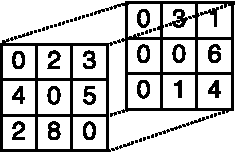
\includegraphics[width=1.7in]{images/tensors.pdf} \label{fig:tens}}
	\qquad
	\qquad
	\subfloat[A view of tensor $T$ with shape $(1\times 2\times 2)$]{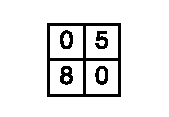
\includegraphics{images/tensors-view.pdf} \label{fig:tensView}}


	\caption{A tensor and a view of it }
	\label{fig:example}
\end{figure}
	
\begin{figure}[!h]

		\[
		\begin{aligned}
		Shape = 
		\begin{bmatrix}
		1 & 2 & 2 
		\end{bmatrix}
		\quad
		Values = 
		\begin{bmatrix}
		5 & 8 
		\end{bmatrix}\\			
		Indexes = 
		\begin{bmatrix}
		0 &  1 & 2 & 0 & 2 & 1
		\end{bmatrix}		
		\quad	
		Flags = 
		\begin{bmatrix}
		1 & 0 & 0
		\end{bmatrix}\\			
		SparseOffsets = 
		\begin{bmatrix}
		0 &  1 & 1
		\end{bmatrix}
		\quad		
		HiddenDimension = 
		\begin{bmatrix}
		0 
		\end{bmatrix}\\			
		\end{aligned}
		\]
		\caption{Parameters defining the view $T_{view}$ in \ref{fig:tensView}}
		\label{eqn:viewParams}
\end{figure}

\subsection{Put a Value}

Several steps are needed to put a new value in a COO array:
\begin{enumerate}
	\item Translate the indexes into the underlying context.
	\item Verify if the value of this indexes is already non null. In this case we can either remove the entry if the new value is 0, or replace the value in the buffer. Nothing else need to be done.
	\item The new value is 0: the indexes and the value are not added in the buffers.
	\item It is a new non-null value: we need to insert the value and the indexes in the buffers. But first we need to ensure that the buffers have enough spaces for the new entries. If not, we need to reallocate them. The new entries are added at the end of the buffers; the sort are not maintained at insertion to avoid sorting the array too often when it is not needed.
\end{enumerate}

\subsection{Get a Sub-Array}

The new parameters make the task easier. Once the indexes resolved and the parameters computed, a new array is created with the current value and indexes buffers and the new parameters. 
